\documentclass[12pt, a4paper]{article}
\usepackage[utf8]{inputenc}
 
\title{Exersice Sheet 1 (Solution)}
\author{Fahad Ashraf , Shabi Turabi}
\date{May 2}

 % --- PACKAGES ---
\usepackage{pgfplots}
\pgfplotsset{width=10cm,compat=1.9}
\usepackage{graphicx}
\graphicspath{ {./images/} }

\begin{document}
 
\begin{titlepage}
\maketitle
\end{titlepage}

\begin{enumerate}
    \setcounter{enumi}{2}
	\item Distribution of weight and height among the citizens genders
	\begin{enumerate}
        \item Scatter plot
        \begin{figure}[h]
            \centering
            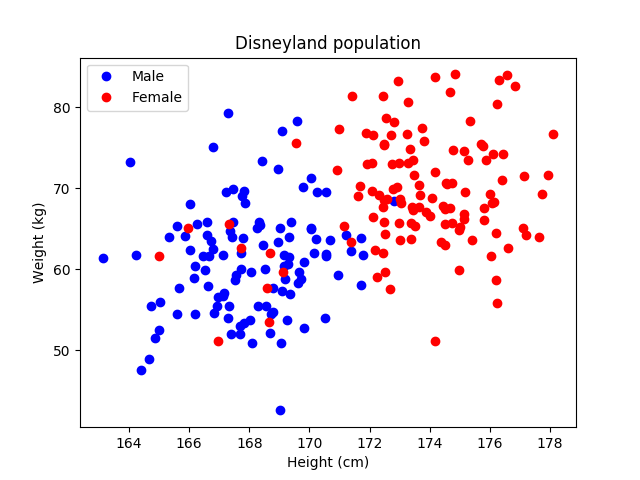
\includegraphics[width=10cm]{scatter_plot}
        \end{figure}
		\item Scatter plot with horizontal line to best seperate male and female citizens
        \begin{figure}[h]
            \centering
            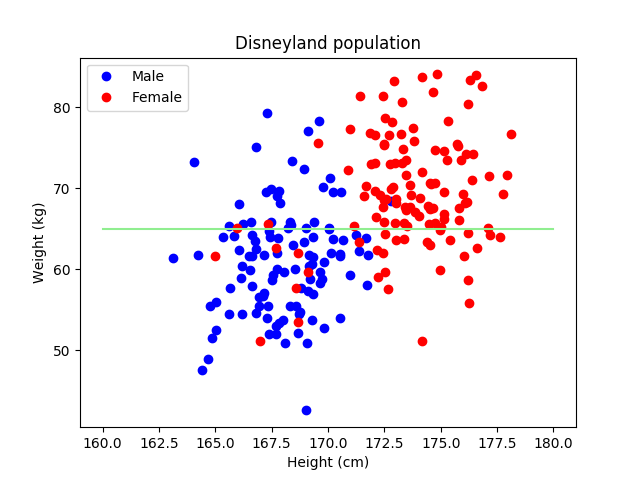
\includegraphics[width=10cm]{scatter_plot_line1}
        \end{figure}
		\item We would say that he/she is his father, but we cannot guarantee that because we do not know the hight value.
		\item Scatter plot with vertical line to best seperate male and female citizens
		\begin{figure}[h]
            \centering
            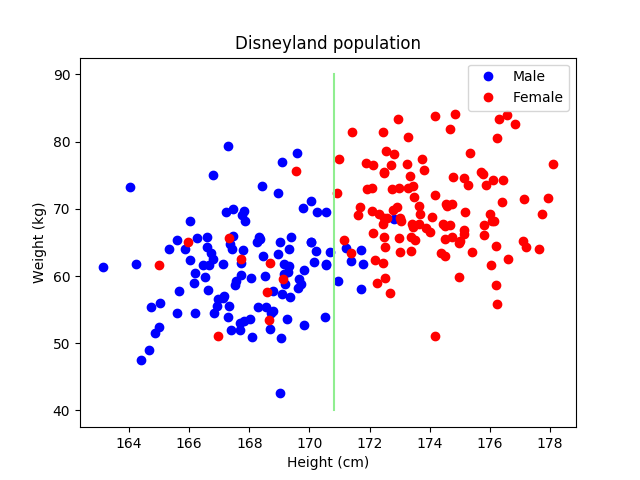
\includegraphics[width=10cm]{scatter_plot_line2}
        \end{figure}
        \item We would say that he/she is his sister, because according to the plot, almost all of the citizens 
        above the hight of 173 are females.
        \item Scatter plot with line to best seperate male and female citizens
		\begin{figure}[h]
            \centering
            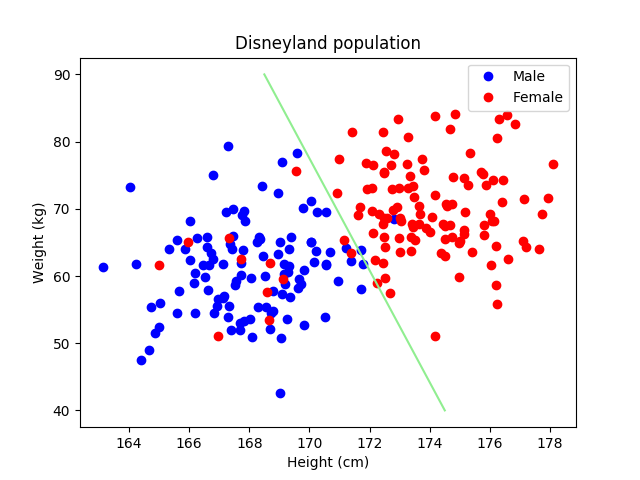
\includegraphics[width=10cm]{scatter_plot_line3}
        \end{figure}
        \item We would classify he/she as a "female" and no we would not classify 
        differently if we use (b) or (d) lines because all of the citizens in that area 
        are females.
	\end{enumerate}
\end{enumerate}
    % \begin{tikzpicture}
    %     \begin{axis}[
    %         enlargelimits=false,
    %     ]
    %     \addplot+[
    %         only marks,
    %         scatter,
    %         mark=halfcircle*,
    %         mark size=2.9pt]
    %     table[meta=ma]
    %     {DWH_Training.csv};
    %     \end{axis}
    % \end{tikzpicture}

\end{document}